\textit{Определение} \textbf{Кликой} в неориентированого графе $\Gamma=(V,E)$ называется множество $C$, такое
что любых двух вершин в $\text{cl}(U)$ существует ребро их соединяющее. \textbf{Максимальной} называется клика, которую
нельзя расширить включением вершин. \textbf{Множеством} клик графа $cl(\Gamma)$ называется множество максимальных графа $\Gamma$.


\textit{Определение} \textbf{Марковские случайные поля} это
вероятностное распределение $p$, заданное на случайных величинах $x_1, \dots,x_n$, образующих
граф $G=(V,E)$, для которых выполняется свойства марковости: \begin{itemize}
    \item пары без ребер условно независимы от прочих переменных $\forall u,v \in V \rightarrow X_u \perp X_v | X_{V \backslash \{i,v\}}$
    \item переменная условна независима от переменных вне связей $x \perp X_{V \backslash adj{V}} |X_{adj(V)} $
    \item любые два подмножества независимы с учетом разделяющего подмножества $X_A \perp X_B | X_S$
\end{itemize}

\begin{figure}[h]
    \centering
    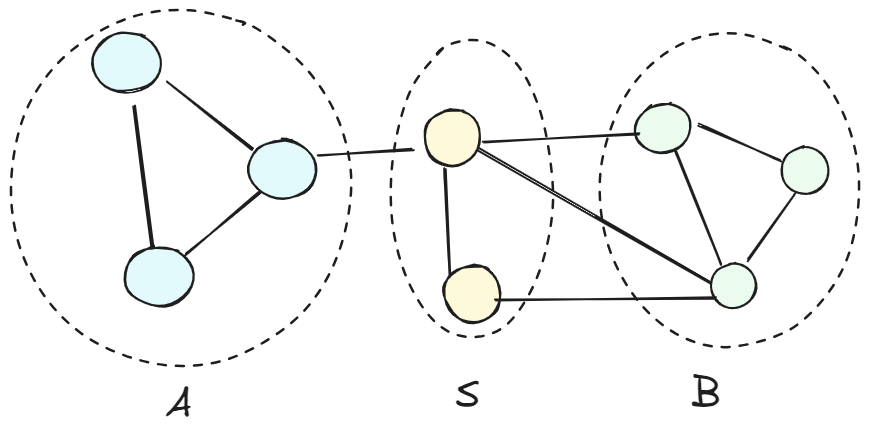
\includegraphics[width=0.5\textwidth]{assets/math/discrete/indep.excalidraw.png}
    \caption{Иллюстрация разделяющего множества для марковских моделей}
    \label{discr_vs_gen}
\end{figure}

Совместное распределение случайных величин $\mathbf{x}$ записывается через функцию $\phi(\mathbf{x})$. 
Марковские свойства, как правило, позволяет факторизовать  $\phi(\mathbf{x})$ на  заданные кликами графа $cl(\Gamma)$:\begin{equation}
    p(x_1, \dots, x_n) = \frac{1}{Z} \prod_{c \in cl{\Gamma}} \phi_c(x_c),
\end{equation} где $Z = \sum_{x_1, \dots}$ - нормализующая переменная.

Частным случаем случайных марковских полей является байесовы сети, задающиеся направленным графом.
Преобразование байесовой сети в случайное марковское поле выполняется \texit{морализацию графа}, заключающегося
в соединение предков узлов. Обратный процесс вычислительно сложен и применяется редко.

\texit{Определение} \textbf{Байесовой сетью} называется ациклический направленный граф $G=(V,E)$ такой, что  
$\forall V \rightarrow x_i \sim p(x_i| \text{parents(i)})$, где $\text{parents(i)}$ - предки узла i.

Такие сети представляют представляют связь между понятиями вероятностно, 
задавая причинно-следственный аппарат как направление в ребре связи графа. 

Факторизация вероятности конфигурации графа задается через цепное правило:
\begin{equation}
    P(X_1, \dots, X_n) = \prod_{i=1}^n P(X_I | \paerents(X_i))
\end{equation}

Для практических задач удобно представлять марковское поле через фактор граф  - двудольный граф
функций и переменных. 

Факторизация вероятности конфигурации такого записывается через произведение двух компонент. Вероятности факторов и :
\begin{equation}
    P(X_1, \dots, X_n) = \prod_{i=1}^n P(X_I | \paerents(X_i))
\end{equation}


\begin{figure}[h]
    \centering
    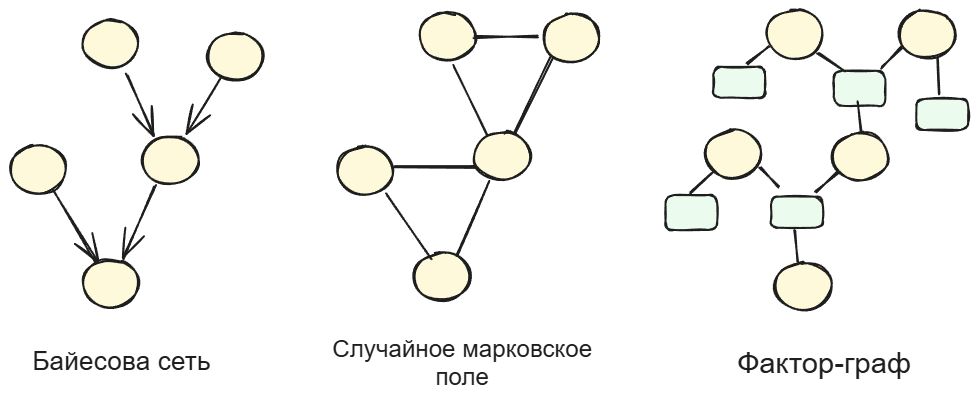
\includegraphics[width=0.5\textwidth]{assets/math/discrete/equivavalence.excalidraw.png}
    \caption{Заданные представления эквивалентны. Выбор представления зависит от постановки}
    \label{factor_graph}
\end{figure}






Выбор графового представления задачи зависит от постановки и выбирается исходя из удобства работы. Так, например, для проверки
независимости переменных, как правило, используются случайные марковские поля, благодаря алгоритмической простоте введения 
разделяющего на ненаправленном графе. 








